\documentclass[conference]{IEEEtran}
\usepackage{amsmath,amssymb,graphicx,booktabs,cite,url,xcolor,bm}
\usepackage{tikz}
\usetikzlibrary{arrows.meta,positioning,calc}
\graphicspath{{../figures/}}
% Simulation numbers quoted in the text of main.tex.
% Sources: results/scenario_metrics.txt and results/evaluation_metrics.txt
% --- standardized scenarios (run_scenarios.m)
\newcommand{\ScN}{50}
\newcommand{\ScRuns}{150}
\newcommand{\ScPulses}{1500}
\newcommand{\ScTint}{0.5}
\newcommand{\ScPointA}{0.26}
\newcommand{\ScPointB}{0.34}
\newcommand{\ScPredA}{1.1}
\newcommand{\ScPredB}{2.8}
% --- held-out evaluation (run_final_evaluation.m)
\newcommand{\EvN}{200}
\newcommand{\EvSucc}{200}
\newcommand{\EvHits}{1964}
\newcommand{\EvPulses}{1964}
\newcommand{\EvTintMean}{0.68}
\newcommand{\EvTintMax}{1.04}
\newcommand{\EvMissMean}{0.35}
\newcommand{\EvMissP}{0.85}
\newcommand{\EvMissMax}{1.68}
\newcommand{\EvLossPulses}{38}
\newcommand{\EvLossMiss}{0.42}
\newcommand{\EvPoint}{0.35}
\newcommand{\EvEst}{0.28}
\newcommand{\EvServo}{0.20}
\newcommand{\EvZ}{1.03}
\newcommand{\EvInR}{99.7}
\newcommand{\EvWorst}{4.0}
\newcommand{\EvTwoLoss}{103}
\newcommand{\AblLeadSucc}{18}
   % every simulation number quoted in the text
\newcommand{\sm}{\sigma_m}
\newcommand{\Reng}{R_{eng}}
\newcommand{\mrad}{\,\mathrm{mrad}}
\newcommand{\rads}{\,\mathrm{rad/s}}
\newcommand{\TODO}[1]{\textcolor{red}{[#1]}}
\makeatletter\newcommand{\tabinput}[1]{\@@input #1 }\makeatother  % expandable \input for table rows

\begin{document}

\title{Due-Time Predictive Fire Control of a Laser Turret\\Against a Maneuvering Aerial Target}

\author{\IEEEauthorblockN{{Ryan Sammy D'Souza (24B2267)}}
\IEEEauthorblockA{ME319: Control Systems, Autumn 2026 --- Assignment 2\\
Department of Mechanical Engineering, Indian Institute of Technology Bombay\\
Code and data: {https://github.com/equuleus0221/guardian-turret}}}

\maketitle

\begin{abstract}
We design the elevation fire-control loop of a point-defense laser turret that must hit a maneuvering target using noisy $20$~Hz radar data that can drop out for up to $0.5$~s. A Kalman filter with a Singer acceleration model estimates the target state in Cartesian coordinates and predicts it over the prescribed horizon $t_p=0.5$~s. Because the laser has no time of flight, we show that the turret must follow each predicted trajectory at its \emph{due time}; tracking the $t_p$-ahead elevation directly leads the target by up to $94$~mrad. The drive model derived from first principles has a lightly damped electromechanical resonance ($56$~rad/s, $\zeta=0.094$) that a low-order model misses. A PI-plus-notch compensator gives a type-2 loop with $57^\circ$ phase margin and $13.8$~dB gain margin. A covariance-based gate decides when to fire. One fixed design intercepts the target in all three standardized scenarios and in \EvSucc{} of \EvN{} randomized held-out engagements, with \EvHits{} of \EvPulses{} pulses inside the $2$~m engagement radius and a mean interception time of \EvTintMean~s.
\end{abstract}

\begin{IEEEkeywords}
target tracking, Kalman filter, Singer model, prediction, notch compensation, type-2 servo, fire control
\end{IEEEkeywords}

\section{Introduction}
The 1944 gun predictors solved a lead problem: a shell needs seconds to arrive, so the gun is aimed where the target will be \cite{mindell}. The Guardian laser turret has a different limiting delay. Light arrives at once, but the fire-control chain is slow: the radar is noisy and sampled at $20$~Hz, it can lose the target for up to $t_{bo}=0.5$~s, and the turret is a $3200$~kg\,m$^2$ inertia driven through a resonant electromechanical drive. The task is to estimate the target motion from range and elevation, predict it over $t_p=0.5$~s, turn the prediction into an elevation reference, track that reference with an LTI compensator, and decide when to release laser pulses that must pass within $\Reng=2$~m of the target.

\textbf{Objectives.} (i) A single estimator, predictor and controller for all cases, without retuning. (ii) Analytical support for every parameter. (iii) A hit on every pulse, as early as possible.

\textbf{Assumptions.} Planar elevation motion; radar co-located with the trunnion; rigid, backlash-free $100{:}1$ gear; trunnion-balanced cradle (no gravity torque); zero-mean Gaussian radar noise with the stated standard deviations; negligible laser propagation and pulse duration. The brief gives no voltage limit, so we assume a drive limit of $\pm1000$~V, about five times the back-emf of the fastest line-of-sight (LOS) rate.

\textbf{Contributions.} (1) An error budget that fixes the loop type and bandwidth before any tuning. (2) The due-time interpretation of the prediction horizon, with a simulation of the alternative. (3) A first-principles plant that exposes a resonance, and a compensator built around it. (4) A firing rule that uses the filter covariance, so the turret holds fire when a radar loss has made the estimate unreliable.

\section{System Architecture and Design}
\begin{figure*}[t]
\centering
\resizebox{0.97\textwidth}{!}{% Fig. 1: (a) elevation-drive schematic, (b) closed-loop block diagram
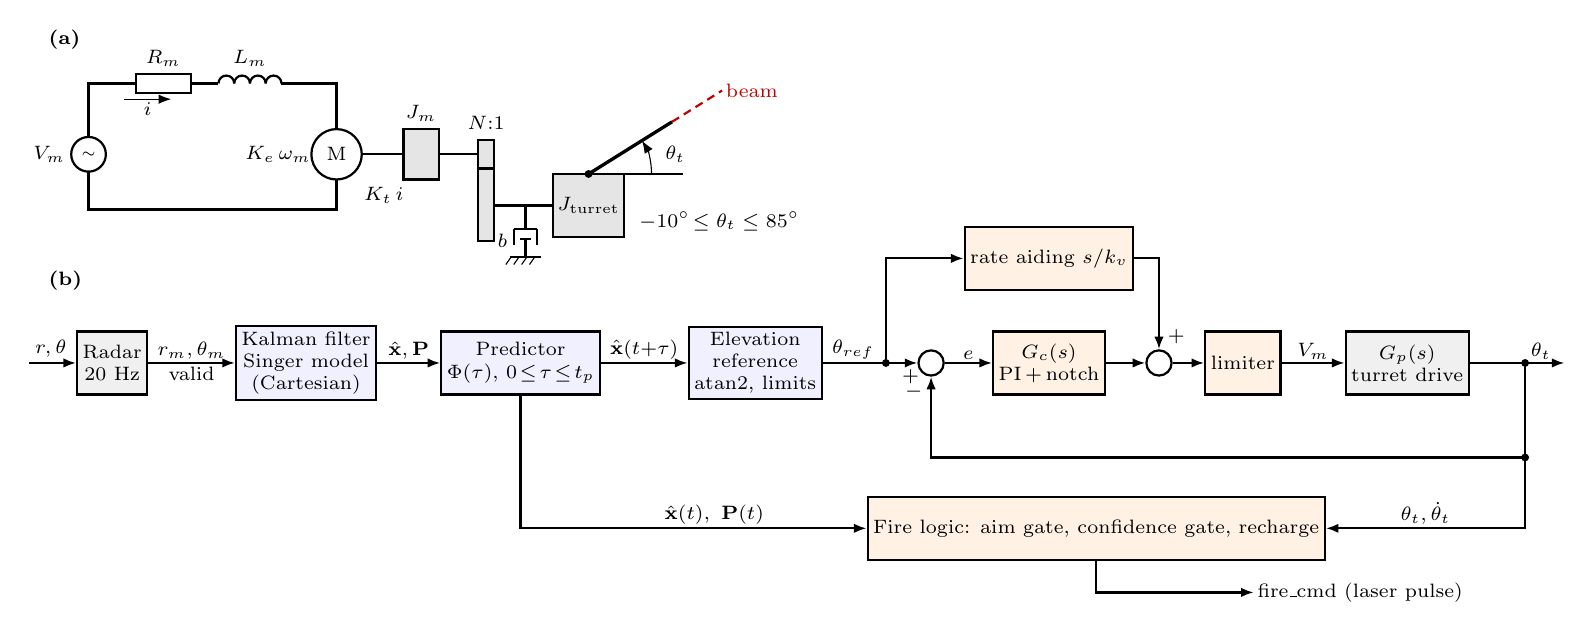
\begin{tikzpicture}[font=\scriptsize, >={Latex[length=1.6mm]},
  blk/.style={draw, thick, minimum height=8mm, align=center, inner sep=2pt, fill=white},
  est/.style={blk, fill=blue!6},
  ctl/.style={blk, fill=orange!10},
  plt/.style={blk, fill=black!6},
  sum/.style={draw, thick, circle, inner sep=0pt, minimum size=3.2mm},
  lbl/.style={font=\scriptsize, inner sep=1pt}]

%% ------------------------------------------------------------- (a) schematic
\begin{scope}[shift={(0,2.55)}]
  \node[lbl, anchor=west, font=\scriptsize\bfseries] at (-0.25,1.55) {(a)};
  % armature circuit
  \draw[thick] (0.3,0.1) circle (2.2mm) node {\tiny$\sim$};
  \node[lbl] at (-0.2,0.1) {$V_m$};
  \draw[thick] (0.3,0.32) -- (0.3,1.0) -- (0.9,1.0);
  \draw[thick] (0.9,0.88) rectangle (1.6,1.12); \node[lbl] at (1.25,1.32) {$R_m$};
  \draw[thick] (1.6,1.0) -- (1.95,1.0);
  \foreach \k in {0,1,2,3} {\draw[thick] (1.95+0.2*\k,1.0) arc (180:0:0.1);}
  \node[lbl] at (2.35,1.32) {$L_m$};
  \draw[thick] (2.75,1.0) -- (3.45,1.0) -- (3.45,0.42);
  \draw[->, thin] (0.75,0.8) -- (1.35,0.8) node[midway, below, lbl] {$i$};
  \draw[thick] (3.45,0.1) circle (3.2mm) node {M};
  \draw[thick] (3.45,-0.22) -- (3.45,-0.6) -- (0.3,-0.6) -- (0.3,-0.12);
  \node[lbl, anchor=west] at (2.25,0.1) {$K_e\,\omega_m$};
  % rotor inertia and gear
  \draw[thick] (3.77,0.1) -- (4.3,0.1);
  \draw[thick, fill=black!10] (4.3,-0.22) rectangle (4.75,0.42); \node[lbl] at (4.52,0.62) {$J_m$};
  \node[lbl] at (4.05,-0.42) {$K_t\,i$};
  \draw[thick] (4.75,0.1) -- (5.25,0.1);
  \draw[thick, fill=black!10] (5.25,-0.08) rectangle (5.45,0.28);
  \draw[thick, fill=black!10] (5.25,-0.08) rectangle (5.45,-1.0);
  \node[lbl] at (5.35,0.5) {$N{:}1$};
  \draw[thick] (5.45,-0.55) -- (6.2,-0.55);
  % damper
  \draw[thick] (5.85,-0.55) -- (5.85,-0.85);
  \draw[thick] (5.7,-0.85) -- (6.0,-0.85); \draw[thick] (5.7,-0.85) -- (5.7,-1.05); \draw[thick] (6.0,-0.85) -- (6.0,-1.05);
  \draw[thick] (5.78,-0.98) -- (5.92,-0.98); \draw[thick] (5.85,-0.98) -- (5.85,-1.2);
  \draw[thick] (5.65,-1.2) -- (6.05,-1.2);
  \foreach \k in {0,1,2,3} {\draw (5.67+0.1*\k,-1.2) -- (5.6+0.1*\k,-1.3);}
  \node[lbl, anchor=east] at (5.66,-1.0) {$b$};
  % turret
  \draw[thick, fill=black!10] (6.2,-0.95) rectangle (7.1,-0.15);
  \node[lbl] at (6.65,-0.55) {$J_{\mathrm{turret}}$};
  \fill (6.65,-0.15) circle (0.5mm);
  \draw[very thick] (6.65,-0.15) -- ++(32:1.25);
  \draw[densely dashed, red!75!black, thick] (6.65,-0.15) ++(32:1.25) -- ++(32:0.75) node[lbl, anchor=west, text=red!75!black] {beam};
  \draw[thin] (6.65,-0.15) -- ++(1.2,0);
  \draw[->, thin] (7.45,-0.15) arc (0:32:0.8);
  \node[lbl] at (7.75,0.1) {$\theta_t$};
  \node[lbl, anchor=west] at (7.25,-0.75) {$-10^\circ\!\le\theta_t\le 85^\circ$};
\end{scope}

%% ---------------------------------------------------------- (b) block diagram
\node[lbl, anchor=west, font=\scriptsize\bfseries] at (-0.25,1.05) {(b)};
\node[plt] (rad) at (0.6,0) {Radar\\$20$ Hz};
\coordinate (tgt) at ($(rad.west)+(-6mm,0)$);
\node[lbl, anchor=south] at ($(rad.west)+(-3.2mm,0.3mm)$) {$r,\theta$};
\node[est, right=11mm of rad] (kf) {Kalman filter\\Singer model\\(Cartesian)};
\node[est, right=8mm of kf] (pred) {Predictor\\$\Phi(\tau)$, $0\!\le\!\tau\!\le\! t_p$};
\node[est, right=11mm of pred] (ref) {Elevation\\reference\\$\operatorname{atan2}$, limits};
\node[sum, right=12mm of ref] (s1) {};
\node[ctl, right=6mm of s1] (gc) {$G_c(s)$\\PI\,+\,notch};
\node[sum, right=5mm of gc] (s2) {};
\node[ctl, right=4mm of s2] (sat) {limiter};
\node[plt, right=8mm of sat] (gp) {$G_p(s)$\\turret drive};
\node[ctl] (fire) at ($(gc)+(6mm,-21mm)$) {Fire logic: aim gate, confidence gate, recharge};
\node[ctl, above=5mm of gc] (ff) {rate aiding $s/k_v$};
\coordinate (tapr) at ($(ref.east)+(8mm,0)$);
\coordinate (tapo) at ($(gp.east)+(7mm,0)$);

\draw[->, thick] (tgt) -- (rad);
\draw[->, thick] (rad) -- node[above, lbl] {$r_m,\theta_m$} node[below, lbl] {valid} (kf);
\draw[->, thick] (kf) -- node[above, lbl] {$\hat{\mathbf x},\mathbf P$} (pred);
\draw[->, thick] (pred) -- node[above, lbl] {$\hat{\mathbf x}(t{+}\tau)$} (ref);
\draw[->, thick] (ref) -- node[above, lbl, pos=0.32] {$\theta_{ref}$} (s1);
\node[lbl] at ($(s1)+(-2.6mm,-1.8mm)$) {$+$};
\draw[->, thick] (s1) -- node[above, lbl] {$e$} (gc);
\draw[->, thick] (gc) -- (s2);
\draw[->, thick] (s2) -- (sat);
\draw[->, thick] (sat) -- node[above, lbl] {$V_m$} (gp);
\draw[->, thick] (gp.east) -- ++(12mm,0) node[above, lbl, pos=0.75] {$\theta_t$};
\fill (tapo) circle (0.5mm);
\draw[->, thick] (tapo) |- ($(s1)+(0,-12mm)$) -- (s1);
\node[lbl] at ($(s1)+(-2.2mm,-3.6mm)$) {$-$};
\fill (tapr) circle (0.5mm);
\draw[->, thick] (tapr) |- (ff);
\draw[->, thick] (ff) -| (s2);
\node[lbl] at ($(s2)+(2.2mm,3.4mm)$) {$+$};
\draw[->, thick] (pred.south) |- node[above, lbl, pos=0.78] {$\hat{\mathbf x}(t),\ \mathbf P(t)$} (fire.west);
\fill ($(tapo)+(0,-12mm)$) circle (0.5mm);
\draw[->, thick] ($(tapo)+(0,-12mm)$) |- node[above, lbl, pos=0.75] {$\theta_t,\dot\theta_t$} (fire.east);
\draw[->, thick] (fire.south) -- ++(0,-4mm) -- ++(20mm,0) node[right, lbl] {fire\_cmd (laser pulse)};
\end{tikzpicture}
}
\caption{(a) Elevation drive: armature circuit, rotor, $100{:}1$ gear, turret with viscous damping. (b) Predictive-feedback architecture. Blue: estimation and prediction; orange: control and firing; grey: physical system.}
\label{fig:arch}
\end{figure*}

Fig.~\ref{fig:arch} shows the drive and the information flow. Each radar sample $(r_m,\theta_m)$ updates the target state estimate $\hat{\mathbf x}$ and its covariance $\mathbf P$. The predictor propagates the estimate to any time ahead. The elevation of the predicted position is the reference of a feedback loop around the turret drive. The fire logic compares the beam with the estimated target position.

\subsection{Error budget}
A pulse hits if the beam passes within $\Reng$ of the target, so the pointing tolerance is $\Reng/r$: $2.5$~mrad at $800$~m and $1.0$~mrad at $2000$~m. Three numbers follow from the target envelope ($v_{max}=150$~m/s, $a_{max}=20$~m/s$^2$):
\begin{itemize}
\item Radar cross-range noise is $r\sigma_\theta=0.28$--$0.70$~m, already below $\Reng$; range noise ($1$~m) is along the beam and does not move the beam off the target. Filtering is needed mainly for velocity and acceleration, i.e. for prediction.
\item The LOS rate reaches $\omega_{L}=v_{max}/r_{min}=0.19\rads$. A type-1 servo would need a velocity constant $K_v\ge190$~s$^{-1}$ to hold $1$~mrad, which the drive resonance forbids. The loop must be type~2.
\item The LOS acceleration is bounded by $\alpha_{L}\le a_{max}/r+v_{max}^2/r^2\le0.060$~rad/s$^2$. A type-2 loop with acceleration constant $K_a$ leaves a miss of $r\alpha_L/K_a\le(a_{max}+v_{max}^2/r)/K_a$, so $K_a\approx45$~s$^{-2}$ keeps the servo share near $1$~m in the worst case.
\end{itemize}

\subsection{What the prediction horizon is for}
\label{sec:due}
The predictor issues, at time $t$, a trajectory $\hat{\mathbf x}(t+\tau\,|\,t)$ for $0\le\tau\le t_p$. Its end point gives the future elevation reference $\theta_p(t)=\operatorname{atan2}(\hat y(t+t_p|t),\hat x(t+t_p|t))$, the angle at which the turret should be \emph{at time $t+t_p$}. If the turret instead tracked $\theta_p(t)$ at time $t$, it would lead the target by $\omega_L t_p$, up to $94$~mrad or $75$~m at $800$~m, and with zero time of flight no pulse could satisfy $\Reng$ unless the LOS rate were nearly zero. Section~\ref{sec:eval} confirms this: that design intercepts only \AblLeadSucc\% of the cases.

We therefore execute each predicted trajectory at its due time. Let $t_k\le t$ be the time of the newest radar sample. The reference is
\begin{equation}
\theta_{ref}(t)=\operatorname{atan2}\big(\hat y(t|t_k),\hat x(t|t_k)\big),\quad t-t_k\le t_p .
\label{eq:ref}
\end{equation}
A new sample supersedes the trajectory issued before it. In normal operation $t-t_k<50$~ms. During a radar loss the turret keeps flying the last issued trajectory, and since $t_{bo}\le t_p$ it never runs past the end of it. The horizon $t_p$ is thus the validity window of a prediction, and it equals the longest loss the system must ride through. Delaying $\theta_p$ by $t_p$ was also rejected: it always points with $0.5$~s-old information, and the measured $t_p$-ahead prediction error ($2.8$~m RMS in Scenario~B) exceeds $\Reng$.

\section{Mathematical Modeling}
\subsection{Turret elevation drive}
With motor speed $\omega_m=N\dot\theta_t$ and all inertia referred to the trunnion,
\begin{align}
J_{eq}\ddot\theta_t+b\,\dot\theta_t&=NK_t\,i, \qquad J_{eq}=J_{turret}+N^2J_m, \label{eq:mech}\\
L_m\,\frac{di}{dt}+R_m i&=V_m-NK_e\dot\theta_t . \label{eq:elec}
\end{align}
The rotor contributes $N^2J_m=2000$~kg\,m$^2$, more than the turret itself ($1200$~kg\,m$^2$), so $J_{eq}=3200$~kg\,m$^2$. Eliminating $i$,
\begin{align}
G_p(s)=\frac{\theta_t(s)}{V_m(s)}&=\frac{NK_t}{s\big[(J_{eq}s+b)(L_ms+R_m)+N^2K_tK_e\big]}\nonumber\\
&=\frac{k_v\,\omega_p^2}{s\,(s^2+2\zeta_p\omega_ps+\omega_p^2)},
\label{eq:Gp}
\end{align}
with $k_v=NK_t/(bR_m+N^2K_tK_e)=9.985\times10^{-4}$~rad/s per volt, $\omega_p=55.94\rads$ and $\zeta_p=0.0936$. Numerically, $G_p(s)=1000/(320s^3+3350s^2+1\,001\,500\,s)$. The complex poles at $-5.23\pm j55.7$ are an exchange of energy between the reflected inertia and the armature inductance through the back-emf. They exist because the electrical time constant $L_m/R_m=0.1$~s is much longer than the electromechanical one, $J_{eq}R_m/(N^2K_tK_e)=3.2$~ms; dropping $L_m$, as is common for small motors, would hide them and predict a well-damped first-order drive. Equations (\ref{eq:mech})--(\ref{eq:elec}) are linear between the stops and below the voltage limit, and with a balanced cradle they do not depend on the operating elevation, so (\ref{eq:Gp}) is the small-perturbation model at every operating point. \texttt{turret\_plant.m} implements (\ref{eq:mech})--(\ref{eq:elec}) with inelastic stops at $-10^\circ$ and $+85^\circ$; its simulated steady speed and ringing frequency agree with (\ref{eq:Gp}) within $0.1$\%.

\subsection{Target model and state estimation}
The target moves in straight lines when it does not maneuver, which is linear in Cartesian coordinates but not in $(r,\theta)$. We therefore estimate $\mathbf x=[x\ v_x\ a_x\ y\ v_y\ a_y]^T$ and model each axis by the Singer process \cite{singer,lijilkov}
\begin{equation}
\dot p=v,\quad \dot v=a,\quad \dot a=-a/\tau_m+w,\quad S_w=2\sm^2/\tau_m ,
\end{equation}
in which acceleration is a zero-mean random process with standard deviation $\sm$ and correlation time $\tau_m$. Over an interval $T$ this gives $\mathbf x_{k+1}=\bm\Phi(T)\mathbf x_k+\mathbf w_k$ with, per axis and $\beta=1/\tau_m$,
\begin{equation}
\bm\Phi_1(T)=\begin{bmatrix}1&T&(\beta T-1+e^{-\beta T})/\beta^2\\0&1&(1-e^{-\beta T})/\beta\\0&0&e^{-\beta T}\end{bmatrix}
\label{eq:Phi}
\end{equation}
and the closed-form $\mathbf Q(T)$ of \cite{singer}. The model has two parameters and both come from the problem data. A vector uniformly distributed in a disc of radius $a_{max}$ has a per-axis standard deviation $\sm=a_{max}/2=10$~m/s$^2$. A weave that stays inside the velocity and range envelope has a period of a few seconds, so $\tau_m=2$~s. A constant-velocity model would be simpler, but an unmodeled $20$~m/s$^2$ acceleration displaces the target by $\tfrac12a_{max}t_{bo}^2=2.5$~m during a loss, more than $\Reng$.

The measurement is converted to Cartesian form, $\mathbf z=[r_m\cos\theta_m\ \ r_m\sin\theta_m]^T=\mathbf H\mathbf x+\mathbf n$, with covariance rotated into the LOS frame \cite{lerro}:
\begin{equation}
\mathbf R=\mathbf J\begin{bmatrix}\sigma_r^2&0\\0&\sigma_\theta^2\end{bmatrix}\mathbf J^T,\quad
\mathbf J=\begin{bmatrix}\cos\theta_m&-r_m\sin\theta_m\\ \sin\theta_m&r_m\cos\theta_m\end{bmatrix}.
\end{equation}
The conversion bias is of order $r\sigma_\theta^2/2<10^{-4}$~m and is ignored, so a linear Kalman filter suffices \cite{barshalom}: time update $\hat{\mathbf x}^-=\bm\Phi\hat{\mathbf x}$, $\mathbf P^-=\bm\Phi\mathbf P\bm\Phi^T+\mathbf Q$; gain $\mathbf K=\mathbf P^-\mathbf H^T(\mathbf H\mathbf P^-\mathbf H^T+\mathbf R)^{-1}$; update $\hat{\mathbf x}=\hat{\mathbf x}^-+\mathbf K(\mathbf z-\mathbf H\hat{\mathbf x}^-)$ with the Joseph form for $\mathbf P$. The filter starts at the first sample with velocity variance $v_{max}^2/2$ and acceleration variance $\sm^2$ per axis. The time update runs at every controller call; the measurement update runs only when \texttt{meas\_valid} flags a new sample. A radar loss therefore needs no special mode: the estimate coasts on (\ref{eq:Phi}) and $\mathbf P$ grows.

\subsection{Prediction and elevation reference}
The predicted state is $\hat{\mathbf x}(t+\tau|t_k)=\bm\Phi(t+\tau-t_k)\hat{\mathbf x}_k$. Setting $\tau=t_p$ gives $\theta_p$; setting $\tau=0$ gives the due-time reference (\ref{eq:ref}), which is limited to $[-9.5^\circ,84.5^\circ]$ to stay off the stops. The predicted LOS rate is $\dot\theta_{ref}=(\hat x\hat v_y-\hat y\hat v_x)/(\hat x^2+\hat y^2)$.

\subsection{Closed-loop model}
With $L(s)=G_c(s)G_p(s)$, $S=1/(1+L)$ and $T=L/(1+L)$, the servo error $e=\theta_{ref}-\theta_t$ under feedback alone is $e=S\,\theta_{ref}$. Adding the rate-aiding voltage $V_{ff}=\dot\theta_{ref}/k_v$ outside the loop, ahead of the notch $N(s)$, gives
\begin{equation}
e=S\Big[1-\tfrac{sNG_p}{k_v}\Big]\theta_{ref}=S\,\frac{s\,(s+2\zeta_d\omega_p)}{s^2+2\zeta_d\omega_ps+\omega_p^2}\,\theta_{ref}.
\label{eq:err}
\end{equation}
The pointing error splits into an estimation part and a servo part,
\begin{equation}
\theta_t-\theta=(\theta_{ref}-\theta)-e .
\label{eq:split}
\end{equation}

\section{Controller Design and Analysis}
\subsection{Compensator}
The compensator is designed by loop shaping on the Bode diagram and checked on the root locus \cite{franklin}:
\begin{equation}
G_c(s)=K_p\,\frac{s+z_i}{s}\cdot\frac{s^2+2\zeta_p\omega_ps+\omega_p^2}{s^2+2\zeta_d\omega_ps+\omega_p^2}.
\label{eq:Gc}
\end{equation}

\emph{Notch.} At resonance the plant gain is magnified by $1/(2\zeta_p)=5.3$ ($14.6$~dB). With a PI alone, $|L(j\omega_p)|\approx K_pk_v/(2\zeta_p\omega_p)$, so a $6$~dB margin at the resonance requires a crossover $\omega_c\approx K_pk_v\le\zeta_p\omega_p=5.2\rads$, which cannot deliver the required $K_a$. With the gains chosen below and no notch, the loop is unstable (a pole pair with real part $+2.1$). The notch replaces the plant damping $\zeta_p$ by $\zeta_d=0.7$.

\emph{Crossover and PI zero.} The loop becomes $L(s)=K_p(s+z_i)k_v\omega_p^2/[s^2(s^2+2\zeta_d\omega_ps+\omega_p^2)]$. Its phase margin is $90^\circ$ minus the lag of the damped pair, $\phi_d=\tan^{-1}\!\frac{2\zeta_d\,\omega_c/\omega_p}{1-(\omega_c/\omega_p)^2}$, minus the lag of the PI, $\tan^{-1}(z_i/\omega_c)$. We choose $\omega_c=15\rads$, about a quarter of $\omega_p$, where $\phi_d=22.0^\circ$, and $z_i=\omega_c/5=3\rads$, which costs $11.3^\circ$. The predicted margin is $90-22.0-11.3=56.7^\circ$. Unit loop gain at $\omega_c$ gives $K_p=14\,748$~V/rad, and
\begin{equation}
K_a=\lim_{s\to0}s^2L(s)=K_pz_ik_v=44.2~\mathrm{s}^{-2},
\end{equation}
which meets the budget of Section~II-A. A crossover of $20\rads$ was rejected: it leaves only $4.9$~dB of gain margin if the resonance is $10$\% low.

\begin{figure*}[t]
\centering
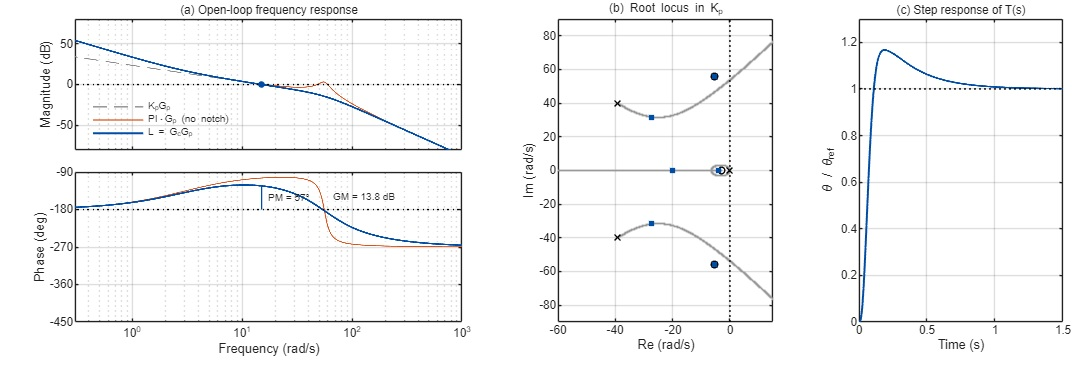
\includegraphics[width=\textwidth]{fig_design.pdf}
\caption{(a) Loop frequency response; without the notch the resonance peak crosses $0$~dB. (b) Root locus in $K_p$ ($\times$ open-loop poles, $\circ$ zeros, squares: design gain). The plant resonance is cancelled by the notch zeros. (c) Unit step response of $T(s)$.}
\label{fig:design}
\end{figure*}

\subsection{Stability and transient response}
Fig.~\ref{fig:design} shows the computed loop. The phase margin is $56.7^\circ$ at $15.0\rads$, the gain margin $13.8$~dB at $53.8\rads$, and the delay margin $66$~ms, far above the $1$~ms controller step. The sensitivity peaks are $M_s=1.46$ and $M_t=1.19$. The closed-loop poles are $-3.97$, $-19.9$ and $-27.2\pm j31.8$ ($\zeta=0.65$); the step response has $16.7$\% overshoot (from the PI zero), a $0.067$~s rise time and a $0.79$~s settling time, and the $-3$~dB bandwidth is $29\rads$. Moving the plant resonance by $\pm10$\% with the notch fixed leaves the phase margin at $56$--$57^\circ$ and the gain margin at $7.5$~dB or more; at $-20$\% the loop is still stable with $3.1$~dB.

The cancelled pair $-5.23\pm j55.7$ remains a mode of the plant. It does not appear in $T(s)$, but any voltage that bypasses the notch excites it and it then decays with a $0.19$~s time constant. This matters for the limiter, below.

\subsection{Steady-state tracking}
The loop is type~2: zero steady-state error for a constant elevation and for a constant LOS rate, and $e_{ss}=\alpha_L/K_a$ for a constant LOS acceleration, i.e. $0.45$~mrad at a typical $0.02$~rad/s$^2$ and $1.36$~mrad at the bound, which occurs at $r_{min}$ where $2.5$~mrad is allowed. With rate aiding, (\ref{eq:err}) has a third zero at the origin, so the error for constant LOS acceleration also vanishes. Rate aiding does not change $L(s)$, hence none of the margins; the feedback loop alone already meets the budget, and Section~\ref{sec:eval} reports the design with rate aiding removed.

\subsection{Noise, prediction error and measurement loss}
By (\ref{eq:split}), reference jitter reaches the beam through $T(s)$, whose noise bandwidth is $37\rads$, below the radar Nyquist frequency ($63\rads$); the $20$~Hz steps of the estimate are smoothed and the tracking voltage stays near $30$~V RMS. The estimation part is set by the filter: with $\sm=10$~m/s$^2$ its steady-state cross-range standard deviation is about $0.3$~m, between the raw radar value and a slower filter that would lag maneuvers.

During a loss of duration $t$ the estimate coasts. If the target changes its acceleration by $\Delta a$ at the onset, the position error grows as $\tfrac12\Delta a\,t^2$: $1.25$~m for $\Delta a=10$~m/s$^2$ after $0.5$~s. This is a limit of the information available, not of the controller. The filter covariance grows accordingly, and the fire logic uses it.

\subsection{Limits: voltage, integrator and elevation stops}
Acquisition is a $0.3$~rad step, for which the linear loop would ask for $4.6$~kV. Three provisions handle this. (i) The $\pm900$~V limiter acts on the PI output, \emph{upstream} of the notch, so the notch also filters the clipped command; clipping after the notch excited the resonance during acquisition in simulation. (ii) The integrator runs only for $|e|\le2$~mrad and while the limiter is inactive, which removes the slow overshoot tail of the PI zero after a slew; all normal tracking is inside this band, where the loop is exactly (\ref{eq:Gc}). Rate aiding makes this safe: without it, the proportional part alone can settle outside a small band at high LOS rates. (iii) The reference is clipped $0.5^\circ$ inside the stops.

\subsection{Fire logic}
The estimated miss if the laser fired now is the perpendicular distance from the estimated target to the beam, $\hat d=-\hat x\sin\theta_t+\hat y\cos\theta_t$, with standard deviation $\sigma_d=(\mathbf h\mathbf P_{pos}\mathbf h^T)^{1/2}$, $\mathbf h=[-\sin\theta_t\ \cos\theta_t]$. Let $d_g=\max(|\hat d|,|\hat d+\dot{\hat d}\tau_f|)$ with $\tau_f=20$~ms, which requires the beam to dwell on the target instead of sweeping through it. A pulse is requested when
\begin{equation}
d_g\le d_{aim}=0.5~\mathrm{m}\quad\text{and}\quad d_g+\kappa\sigma_d\le\Reng,\quad\kappa=3,
\end{equation}
at least $1$~s after the previous pulse and after four radar samples. The second condition is a $3\sigma$ bound on the true miss. It needs no blackout flag: as $\sigma_d$ grows during a loss, the gate closes by itself. Table~\ref{tab:par} collects the design parameters.

\begin{table}[t]
\caption{Design parameters and their basis}
\label{tab:par}
\centering
\footnotesize
\setlength{\tabcolsep}{3pt}
\begin{tabular}{@{}lll@{}}
\toprule
Parameter & Value & Basis\\
\midrule
$\sm$ & $10$ m/s$^2$ & $a_{max}/2$, uniform in a disc\\
$\tau_m$ & $2$ s & weave period of a few seconds\\
$\omega_c$ & $15\rads$ & $\approx\omega_p/4$; gives $K_a=44$~s$^{-2}$\\
$z_i$ & $3\rads$ & $\omega_c/5$, costs $11^\circ$ of phase\\
$\zeta_d$ & $0.7$ & well-damped replacement poles\\
$K_p$ & $14\,748$ V/rad & $|L(j\omega_c)|=1$\\
$V_{lim}$, $V_{max}$ & $900$, $1000$ V & $\approx5\times$ largest back-emf (assumed)\\
$e_{int}$ & $2$ mrad & tolerance at $r_{min}$; $\gg$ tracking error\\
$d_{aim}$ & $0.5$ m & $\Reng/4$\\
$\kappa$ & $3$ & $3\sigma$ bound on the miss\\
$\tau_f$ & $20$ ms & dwell; a few controller steps\\
\bottomrule
\end{tabular}
\end{table}

\section{Simulation and Results}
The complete system is simulated in MATLAB with the three prescribed functions, a fixed-step RK4 integration of the plant at $1$~ms and the controller called every step. The turret starts at $\theta_t=0$. Scenario~A is a straight $100$~m/s pass. Scenario~B adds, from $t=1$~s, accelerations $12\sin1.3\tau$ and $15\sin2\tau$~m/s$^2$ in $x$ and $y$ (peak $19.0$~m/s$^2$). Scenario~C is B with the radar lost from $1.0$ to $1.5$~s. The generator checks range, speed and acceleration limits for every trajectory (Fig.~\ref{fig:geom}).
\begin{figure}[t]
\centering
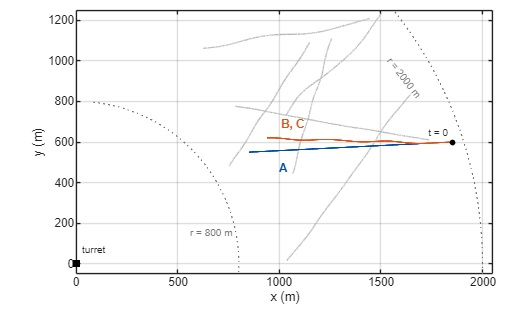
\includegraphics[width=\columnwidth]{fig_geometry.pdf}
\caption{Engagement geometry. Scenario A (blue), B and C (red), and six of the randomized evaluation trajectories (grey).}
\label{fig:geom}
\end{figure}

\begin{figure*}[t]
\centering
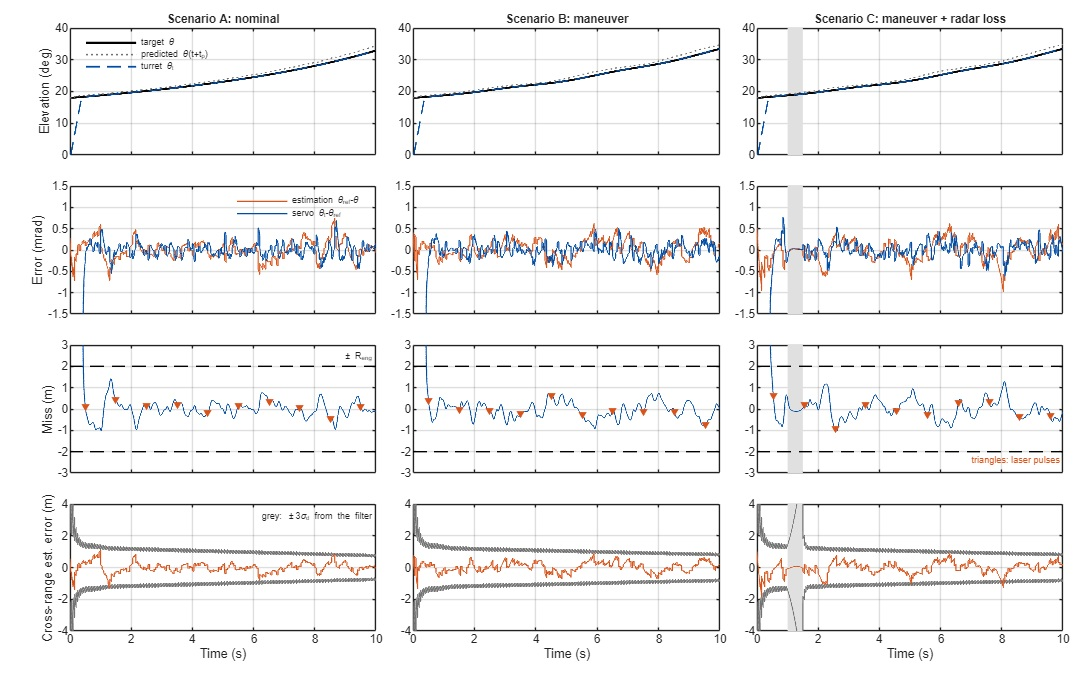
\includegraphics[width=\textwidth]{fig_scenarios.pdf}
\caption{Standardized scenarios, one run each. Row 1: target, $t_p$-ahead predicted and turret elevation. Row 2: the two parts of the pointing error in (\ref{eq:split}). Row 3: distance between beam and target, with the laser pulses. Row 4: cross-range estimation error against the filter's own $\pm3\sigma_d$. Grey band: radar loss.}
\label{fig:scen}
\end{figure*}

\begin{table}[t]
\caption{Standardized scenarios: \ScN{} noise realisations each; tracking statistics for $t\ge2$~s}
\label{tab:scen}
\centering
\footnotesize
\setlength{\tabcolsep}{3.5pt}
\begin{tabular}{@{}lccc@{}}
\toprule
 & A & B & C\\
\midrule
\tabinput{../results/tab_scenarios.tex}
\bottomrule
\end{tabular}
\end{table}

Fig.~\ref{fig:scen} and Table~\ref{tab:scen} give the results. The turret slews at the voltage limit, settles without ringing, and the first pulse is released after about \ScTint~s, before the earliest possible radar loss. All \ScPulses{} pulses of the \ScRuns{} runs hit. Three observations connect the results to the analysis.

\emph{Estimation dominates.} In all scenarios the estimation part of the pointing error exceeds the servo part, as intended by the budget: the loop is fast enough that the beam error is set by what the radar can know.

\emph{Maneuvers.} From A to B the pointing error rises from \ScPointA{} to \ScPointB~mrad RMS. The $t_p$-ahead prediction error rises much more, from \ScPredA{} to \ScPredB~m, because prediction extrapolates an estimated acceleration over $0.5$~s. This is the measured basis for pointing with the newest estimate (Section~\ref{sec:due}).

\emph{Radar loss.} In C the $3\sigma_d$ band opens during the loss and the gate holds fire; the miss stays inside $\Reng$ because the loss falls at the maneuver onset, where the acceleration is still small.

\section{Final Evaluation}
\label{sec:eval}
The instructor's evaluation cases are not available before submission, so the finalized design was tested on \EvN{} randomized engagements that played no part in the design (design choices used $40$ other cases). Each case draws a random initial range ($1450$--$1950$~m), elevation, speed and heading, a two-frequency maneuver in each axis starting within the first $2$~s and scaled to $60$--$98$\% of $a_{max}$, and one or two radar losses of $0.2$--$0.5$~s with onset after $1$~s; trajectories violating the envelope are rejected. \EvTwoLoss{} cases have two losses.

\begin{figure*}[t]
\centering
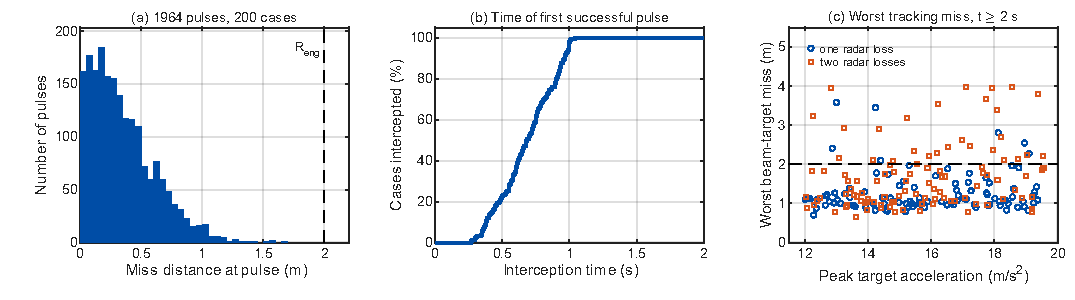
\includegraphics[width=\textwidth]{fig_evaluation.pdf}
\caption{Held-out evaluation, \EvN{} randomized cases. (a) Miss distance of every pulse. (b) Distribution of interception time. (c) Worst beam--target distance per case after acquisition; excursions beyond $\Reng$ occur at the end of radar losses under hard maneuvers, when the gate withholds fire.}
\label{fig:eval}
\end{figure*}

\emph{Interception.} All \EvSucc{} of \EvN{} cases are intercepted, and \EvHits{} of \EvPulses{} pulses are hits (Fig.~\ref{fig:eval}). The interception time is \EvTintMean~s on average and at most \EvTintMax~s; it is set by the $0.14$--$0.8$~rad acquisition slew at the voltage limit.

\emph{Accuracy.} The miss at the pulse is \EvMissMean~m on average, \EvMissP~m at the 95th percentile and \EvMissMax~m at worst. \EvLossPulses{} pulses were released early in a radar loss; their mean miss is \EvLossMiss~m.

\emph{Consistency.} The RMS pointing error is \EvPoint~mrad (estimation \EvEst, servo \EvServo). The cross-range error divided by the filter's own $\sigma_d$ has a standard deviation of \EvZ{} (ideal $1$), so the confidence gate rests on an honest covariance even though the true maneuvers are deterministic sinusoids and not Singer processes. The beam is within $\Reng$ for \EvInR\% of the time after acquisition; the worst excursion, \EvWorst~m, occurs at the end of a loss (Fig.~\ref{fig:eval}c). Its size is what $\tfrac12\Delta a\,t^2$ of Section~IV-D gives when the target reverses its acceleration during the loss ($\Delta a$ up to $2a_{max}$, i.e. $5$~m). No pulse is released there.

\begin{table}[t]
\caption{Design alternatives on $100$ of the held-out cases}
\label{tab:abl}
\centering
\footnotesize
\setlength{\tabcolsep}{2.5pt}
\begin{tabular}{@{}p{3.55cm}ccccc@{}}
\toprule
Design & \shortstack{Succ.\\(\%)} & \shortstack{Pulse\\hits (\%)} & \shortstack{$t_{int}$\\(s)} & \shortstack{Pulse\\miss (m)} & \shortstack{Track\\RMS (m)}\\
\midrule
\tabinput{../results/tab_ablation.tex}
\bottomrule
\end{tabular}
\end{table}

\emph{Alternatives} (Table~\ref{tab:abl}). Leading the reference by $t_p$ fails in most cases, as argued in Section~\ref{sec:due}. Feedback alone, with a linear PI, is equally reliable but intercepts $0.8$~s later because of the overshoot tail. A near-constant-velocity filter still intercepts every case but $4$\% of its pulses miss and its tracking miss more than doubles. Without the confidence gate $5$\% of the pulses miss; many of these are released too early during acquisition, and the recharge time then delays the first hit.

\emph{Stress tests.} A second evaluator, sharing no code with the first, flew $280$ engagements from seven other motion families: straight passes, bang-bang jinks, sustained turns, a full reversal at the onset of a $0.5$~s loss, a $150$~m/s crosser at $810$--$900$~m, elevations up to $84^\circ$, and four or five losses. All were intercepted and all $2661$ pulses hit (worst miss $1.74$~m). Thirteen calling conventions (Euler or RK4, $1$--$10$~ms steps, controller inside RK4 stages, \texttt{meas\_valid} held high, NaN during a loss, turret starting on a stop) gave $390/390$ and $3784/3784$, after one fault was corrected: a repeated pre-loss measurement was fused as current when \texttt{meas\_valid} is held high.

\section{Conclusions}
A Singer-model Kalman filter, due-time execution of its predictions, a PI-plus-notch type-2 loop and a covariance-gated firing rule form one fixed design that intercepted every standardized and every randomized case we generated, with all pulses inside the engagement radius. \emph{Strengths:} each parameter follows from the problem data or from a stated margin; the pointing error is dominated by estimation, as budgeted; radar loss needs no special logic. \emph{Limitations:} (i) the notch cancels the resonance and does not damp it, so performance depends on the model of $\omega_p$ within about $\pm10$\% and on keeping clipped voltages behind the notch; (ii) the $1000$~V limit is our assumption and sets the interception time; (iii) after a long loss under a hard maneuver the beam can leave the engagement radius, and the system then waits; (iv) the results rest on our own test cases with Gaussian noise, and not on the instructor's evaluation set. The factors that most affect performance are the cross-range radar noise, the maneuver jerk during a loss, and the acquisition slew.

\begin{thebibliography}{9}
\bibitem{mindell} D.~A. Mindell, \emph{Between Human and Machine: Feedback, Control, and Computing Before Cybernetics}. Baltimore, MD, USA: Johns Hopkins Univ. Press, 2002.
\bibitem{singer} R.~A. Singer, ``Estimating optimal tracking filter performance for manned maneuvering targets,'' \emph{IEEE Trans. Aerosp. Electron. Syst.}, vol.~AES-6, no.~4, pp.~473--483, Jul. 1970.
\bibitem{lijilkov} X.~R. Li and V.~P. Jilkov, ``Survey of maneuvering target tracking. Part~I: Dynamic models,'' \emph{IEEE Trans. Aerosp. Electron. Syst.}, vol.~39, no.~4, pp.~1333--1364, Oct. 2003.
\bibitem{lerro} D.~Lerro and Y.~Bar-Shalom, ``Tracking with debiased consistent converted measurements versus EKF,'' \emph{IEEE Trans. Aerosp. Electron. Syst.}, vol.~29, no.~3, pp.~1015--1022, Jul. 1993.
\bibitem{barshalom} Y.~Bar-Shalom, X.~R. Li, and T.~Kirubarajan, \emph{Estimation with Applications to Tracking and Navigation}. New York, NY, USA: Wiley, 2001.
\bibitem{franklin} G.~F. Franklin, J.~D. Powell, and A.~Emami-Naeini, \emph{Feedback Control of Dynamic Systems}, 8th~ed. New York, NY, USA: Pearson, 2019.
\end{thebibliography}

\clearpage
\appendices
\section{Use of AI and Computational Tools}
\textbf{Tools.} Claude (Anthropic), used as a coding agent in Claude Code; ChatGPT (OpenAI), used by the author to cross-check the hand derivations and to help write the design decision log; MATLAB R2025a (no toolboxes required); MiKTeX/pdfLaTeX with TikZ.

\textbf{Contribution of each tool.} Claude proposed the architecture, derived the models, wrote all MATLAB code and scripts, ran the simulations through MATLAB, and wrote the first complete draft of this paper, including figures and tables. MATLAB executed every numerical result; no number in the paper was produced by the language model without a script that reproduces it (\texttt{design\_controller.m}, \texttt{run\_scenarios.m}, \texttt{run\_final\_evaluation.m}, \texttt{run\_stress\_tests.m}). The author set the task, directed the work, requested the independent stress tests of Section~VI, and takes responsibility for the submitted design. After the AI's proposal, the author reviewed the principal design decisions and recorded his own reasoning on each (\texttt{design-decisions.md} in the repository) and re-derived parts of the model and controller analysis by hand (\texttt{handwritten/}).

\textbf{AI outputs accepted, modified or rejected.}
\begin{itemize}
\item \emph{Accepted:} first-principles plant (\ref{eq:Gp}), after checking the simulated plant against it (steady speed and ringing frequency); Singer filter with converted measurements, after the consistency test ($\sigma$-normalised error \EvZ); PI-plus-notch structure, after the analytic phase budget $90-22.0-11.3=56.7^\circ$ agreed with the numerically computed margin.
\item \emph{Modified:} crossover reduced from the first proposal of $20$ to $15\rads$ after the $-10$\% resonance test left $4.9$~dB gain margin; fire rule extended from a single confidence threshold to aim, dwell and confidence gates after a pulse was released while the beam swept across the target; voltage limiter moved upstream of the notch after the first version rang the resonance; integrator band and rate aiding added after the linear PI gave a $1.5$~s interception time; new-sample test changed to ``values differ from the last sample used'' after the stress test showed a repeated measurement being fused when \texttt{meas\_valid} is held high ($88$ of $569$ pulses missed in those two conventions before the change, none after).
\item \emph{Rejected:} tracking the $t_p$-ahead reference directly (\AblLeadSucc\% success); delaying the predicted reference by $t_p$ (stale information after a loss); a fire threshold of $|\hat d|+3\sigma_d\le1$~m (first pulse after $2.8$~s on average); PI without a notch (unstable at the required gain); conditional integration without rate aiding ($5$ of $40$ design cases not intercepted); a near-constant-velocity target model (Table~\ref{tab:abl}).
\end{itemize}

\textbf{Validation reasoning.} (1) The plant code is tested against the transfer function, not only derived. (2) Margins are computed from the loop polynomials and cross-checked against the analytic phase budget and a $\pm20$\% resonance sweep. (3) The estimator is judged by whether its covariance matches its actual error, since the fire rule depends on it. (4) Design decisions used $40$ randomized cases; the reported evaluation uses \EvN{} different ones. The standardized scenarios were used to diagnose behaviour, and no parameter was set per scenario. (5) Known gaps are stated in the Conclusions: the voltage limit is an assumption, and the instructor's evaluation cases were not run.
\end{document}
